\chapter{Grundlagen}
\label{chap:grundlagen}
    In diesem Kapitel werden die für diese Thesis relevanten Grundlagen geschaffen, um ein Grundverständnis und 
    fundiertes Wissen über verwendete Technologien zu erlangen und die nachfolgende Recherche, Konzeption und 
    Umsetzung besser verstehen zu können. 

\section{Internet der Dinge}
\label{sec:iot}
    Das \ac{IdD}, im Englischen \ac{IoT}, zählt als eines der Schlagworte in der \ac{IT}. In der Domäne des \acs{IoT} bekommen 
    Gegenstände und Objekte eine eindeutige Identität, die eine Kommunikation miteinander als auch das Entgegennehmen von 
    Befehlen erlaubt. Mit dem \acl{IdD} lassen sich Anwendungen sowie Prozesse automatisieren und Aufgaben erledigen, ohne das 
    von außen Eingegriffen werden muss \cite{bigdatainsider2016}. Die Prozessautomatisierung findet sich im Kontext des 
    \acl{SH} wieder, welches in nachfolgendem Kapitel genauer aufgegriffen wird. 
    \\
    \linebreak
    In der einschlägigen Literatur gibt es für das \acl{IoT} keine allgemeingültige Definition, die alle Anwendungsbereiche abdeckt. 
    Die Definitionen und Auslegungen der Interpretation unterscheiden sich je nach Anwendungsgebiet. Demnach gibt es viele verschiedene 
    Forschungsgruppen, darunter Forscher, Akademiker, Innovatoren, Entwickler und Geschäftsleute, die den Begriff oder die zugrunde liegende 
    Problemstellung definiert haben. Die Ursprünge jedoch sind dem Experten für digitale Innovationen, 
    Kevin Ashton\footnote{Britischer Technologie-Pionier, Mitgründer des Auto-ID Centers am Massachusetts Institute of Technology (MIT). \url{https://de.wikipedia.org/wiki/Kevin_Ashton} (Abgerufen am 22.03.2022)}, 
    zuzuschreiben. 
    \\ 
    Die in der Literatur auffindbaren Definitionen verfolgen zwei Sichtweisen. Zum einen die aktive Sicht, d. h. 
    die Daten sind von Menschen erstellt, zum anderen die passive, bei der die Daten von Dingen, darunter die Sensoren und Aktoren, 
    erstellt werden \cite{Madakam2015}. Eine aus dem Zusammenhang hervorgehende, aus dem wissenschaftlichen Artikel entnommene 
    Definition ist folgende:
    % „Ein offenes und umfassendes Netzwerk intelligenter Objekte, die in der Lage sind, sich automatisch zu organisieren, 
    % Informationen, Daten und Ressourcen auszutauschen und auf Situationen und Veränderungen in der Umgebung zu reagieren 
    % und zu handeln.“
    \pagebreak
    \begin{quote}
        “An open and comprehensive network of intelligent objects that have the capacity to auto-organize, share information, data 
        and resources, reacting and acting in face of situations and changes in the environment” \cite{Madakam2015}
    \end{quote}
    Daraus kann die Ableitung erfolgen, dass der Begriff des \acl{IdD} für die Vernetzung von Gegenständen im privaten Gebrauch sowie 
    von industriellen Geräten und Maschinen über das Internet steht. Damit Geräte individuell angesprochen werden können, werden diese 
    mit einer eindeutigen Identität, genauer einer \ac{IP}-Adresse, im Netzwerk belegt und mit elektronischer Intelligenz ausgestattet \cite{bigdatainsider2016}.
    Darüber können die Netzwerkteilnehmer über das Internet kommunizieren und Prozesse automatisiert erledigen. Die sogenannten 
    \textit{intelligenten Geräte} werden oft mit dem englischen Begriff, \textit{Smart Devices}, betitelt. 
    \\
    \linebreak
    Neben der Kommunikation der Geräte untereinander kann ebenso entweder über das Gerät selbst oder eine zentrale 
    Schnittstelle via Internet interagiert werden. Dadurch sind Objekte und Gegenstände durch einen Benutzer von beliebigen Orten aus  
    auch außerhalb des Netzwerks erreich- und bedienbar. Diese Art und Weise wird in dem zentralen Thema des 
    \acl{SH} verwendet. Die Funktion als auch die Umsetzung wird im Kapitel (\ref{sec:smartHome}) näher beleuchtet.
    \\
    \linebreak
    Das \acl{IdD} ist ein elementarer Baustein der \acs{IT}-Welt. Mit dem \acs{IoT} wird die Vision verfolgt, eine globale 
    Infrastruktur zu erstellen, mit der physische Objekte miteinander vernetzt werden und jeder Zeit zur Verfügung stehen. Das \acl{IoT} 
    kann als globales Netzwerk angesehen werden, indem die Kommunikation zwischen Mensch zu Mensch, Gerät zu Mensch und Gerät zu 
    Gerät ermöglicht wird. Viele Forschungsartikel sprechen von der Verschmelzung der digitalen und 
    physischen Welt.\footnote{Das Internet der Dinge – der digitale Zwilling der Welt. Kompetenzzentrum Öffentliche IT in Kooperation mit dem Fraunhofer Institut. \url{https://www.oeffentliche-it.de/trendsonar-iot} Abgerufen am 23.03.2022.} 
    Die Vereinigung beider Welten ist die Verknüpfung physischer Objekte, die eindeutig identifizierbar sind, mit einer virtuellen 
    Repräsentation in einer vergleichbaren Internet-Struktur. 
    %\pagebreak
    \subsection*{Gesamtbild des \acl{IoT}}
        Der folgenden Abbildung (\ref{pic:mindmap_IoT}) ist zu entnehmen, welche Technologien rund um das \acl{IdD} liegen und in Verbindung damit stehen. 
        \begin{figure}[hbt!]
            \centering
            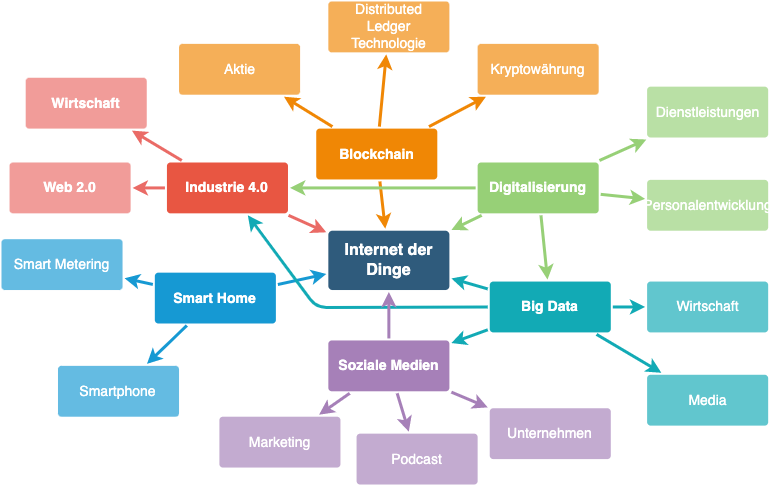
\includegraphics[width=15cm,height=15cm,keepaspectratio]{images/IoT-Mind_Map.png}
            \caption{Technologische Einordnung von IoT \cite{iotmindmap2018}}
            \label{pic:mindmap_IoT}
        \end{figure}
        \\
        \pagebreak
        \linebreak
        Beispielsweise ist das \acs{IoT} eine wesentliche Grundlage für das Themengebiet \textit{Big Data}. Die durch Sensoren 
        und Aktoren erzeugten Daten 
        können eine Grundlage für die Verwendung im Bereich \textit{Big Data} sein. Dabei werden die Datenmengen gespeichert und mithilfe von Mustern 
        und Herangehensweisen des Big Data\footnote{Definition und Funktionsweise von Big Data. \url{https://www.oracle.com/big-data/what-is-big-data/} Abgerufen am 25.03.2022} 
        analysiert. 
        Big Data ist kein Bestandteil dieser Arbeit und wird demnach nicht weiter ausgeführt. Das Beispiel dient lediglich zu Veranschaulichung 
        und Interpretation der oben aufgeführten Abbildung (\ref{pic:mindmap_IoT}).
        \\
        \linebreak
        Eine allgemeine exemplarische Skizzierung eines Systems, welches nach dem \acs{IoT}-Konzept aufgebaut ist, kann der folgenden 
        Abbildung (\ref{pic:skizze_iot}) entnommen werden:
        \begin{figure}[hbt!]
            \centering
            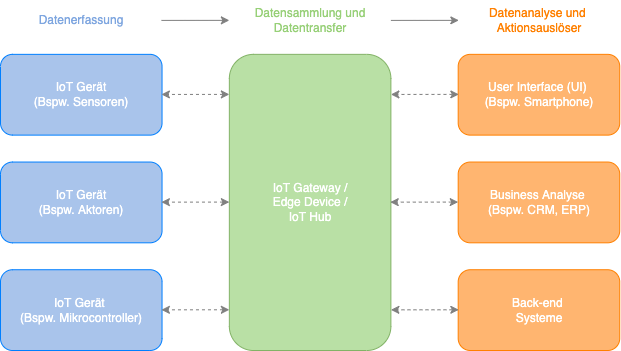
\includegraphics[width=15cm,height=15cm,keepaspectratio]{images/IoT_Grundstruktur.png}
            \caption{Exemplarische Darstellung eines \acs{IoT}-Systems \cite{iotskizze2022}}
            \label{pic:skizze_iot}
        \end{figure}
        \\
        \pagebreak
        \linebreak
        Hierbei werden die jeweiligen Komponenten verdeutlicht, die in einem System zu finden sind. Mit den \textit{IoT-Geräten}, darunter 
        beispielsweise Sensoren und Aktoren, findet die Datenerzeugung statt. Mit dem dahinterstehenden \textit{Gateway} werden die aus den Geräten 
        erzeugten Daten gesammelt und an zentraler Stelle an die Cloud gesendet. Nach der Datensammlung können diese an verschiedene 
        Komponenten zur weiteren Verarbeitung gesendet werden, die durch die Visualisierung über das Smartphone stattfinden kann oder zur Durchführung von 
        Prozessanalysen dient. Ebenso können die Daten an weitere Backend-Systeme zur Weiterverarbeitung übermittelt werden. 

    \subsubsection*{Anwendungsbereiche des \acs{IoT}}
        Grundlegend kann im Bereich des \acl{IoT} zwischen zwei Anwendungsbereichen unterschieden werden. Dies ist zum einen der private Bereich und zum 
        anderen der industrielle. Der private Bereich deckt hauptsächlich die Thematik rund um den Gebrauch von Alltagsgegenständen ab und 
        deren Vernetzung untereinander zur komfortableren und intelligenteren Nutzung der Geräte. Darin inbegriffen sind 
        Gebäudeautomatisierungen und Ereignissteuerungen über das Internet. Diese Funktionen sind Hauptbestandteil des \acl{SH}-Konzeptes, welches 
        in Abschnitt (\ref{sec:aufbau}) genauer aufgegriffen wird. 
        \\
        \linebreak
        Der industrielle Bereich beschäftigt sich mit der Vernetzung von Maschinen und Anlagen miteinander, sodass sich ganze industrielle Prozesse 
        automatisieren lassen und so die Effizienz der Prozess- und Produktionsabläufe gesteigert werden. Die Nutzung des \acs{IoT} im industriellen Bezug 
        ist ein elementarer Bestandteil der heutigen \textit{Industrie 4.0}\footnote{Definition und Beschreibung der Industrie 4.0 \url{https://www.plattform-i40.de/IP/Navigation/EN/Industrie40/WhatIsIndustrie40/what-is-industrie40.html} Abgerufen am 25.03.2022},
        auch bekannt als \textit{\ac{IIoT}}. 
        \\
        Im Rahmen dieser Arbeit wird zwischen den beiden Anwendungsbereichen 
        differenziert und den Fokus auf den privaten Bereich gelegt. 
        \\
        \linebreak
        Mit dem \acl{IdD}-Ansatz gibt es zwei Paradigmen, die in Kombination als auch alleinstehend Anwendung finden. Diese werden im folgenden Abschnitt kurz erläutert.

        \subsubsection*{Edge und Cloud Computing}
            Bei den beiden Paradigmen handelt es sich zum einen um Edge Computing und zum anderen um Cloud Computing. Ziel beider Ansätze ist das 
            Verwalten von Daten bzw. das Arbeiten mit erzeugten Daten.
            \\
            Das Edge Computing verfolgt einen \textit{dezentralen Ansatz}, bei dem die Berechnung und Erhebung der Daten direkt auf dem Gerät durchgeführt wird. %näher bei der Datenerzeugung gehalten wird. 
            Dies bedeutet, dass jedes Gerät über eine eigene Intelligenz verfügt, bei der Daten direkt nach der Erzeugung verarbeitet und gespeichert werden können. 
            Zu einem späteren Zeitpunkt können in Form einer Datenbündelung oder einer Vorauswahl die Informationen an ein Rechenzentrum weitergegeben werden. 
            \begin{quote}
                “Edge computing is different from traditional cloud comput- ing. It is a new computing paradigm that performs computing at the edge 
                of the network. Its core idea is to make computing closer to the source of the data [...]” \cite{Cao2020}
            \end{quote}
            Bei Cloud Computing handelt es sich grundlegend um Bereitstellungen von Computerdiensten, Kapazitäten, Ressourcen und der Rechenleistung über 
            das Internet, die nicht in einem eigenen Rechenzentrum 
            verwaltet und betrieben werden müssen. Die Verwaltung wird dem Anbieter des Cloud Computing überlassen. Hauptsächlich steht dabei die 
            flexible Ressourcennutzung, Skalierung und Verteilung von Rechenleistungen im Vordergrund. In Zusammenhang mit den verfügbaren Ressourcen 
            werden auch verschiedene Modelle, Cloud Typen und diverse Dienste angeboten\footnote{Einblick in die Cloud-Umgebung von dem Anbieter Microsoft. \url{https://azure.microsoft.com/en-us/overview/what-is-cloud-computing/} Abgerufen am 28.03.2022}. 
            Diese werden ihm Rahmen der Arbeit nicht weiter ausgeführt.
            \begin{quote}
                “Cloud computing is a model for enabling ubiquitous, convenient, on-demand network access to a shared pool of configurable 
                computing resources (e.g., networks, servers, storage, applications, and services) that can be rapidly provisioned and 
                released with minimal management effort or service provider interaction.” \cite{Mell2011}
            \end{quote}
            Mit dem Cloud Computing wird im Vergleich zum Edge Computing ein zentraler Ansatz verfolgt, bei dem die erzeugten Daten von den Aktoren und 
            Sensoren direkt an eine zentrale Stelle gelangen. Von dort aus findet die Verarbeitung und Analyse der Daten statt. 
            \\
            Eine Kombination beider Ansätze vereint deren Vorteile und ist als \textit{Hybrid Cloud} bekannt. Diese Konstellation ist in den meisten 
            Architekturen wiederzufinden. 
    
    \subsection{Paradigmen und Kommunikationsmodelle}
        Damit eine umfassende Grundlage im Bereich \acs{IoT} geschaffen wird, behandelt folgender Abschnitt Paradigmen und Kommunikationsmodelle, die 
        in dieser Umgebung verwendet werden. Für die Darstellung dieser Modelle wird eine Literaturquelle genutzt, die ein paar der gängigsten und 
        prägnantesten Architekturen und Modelle abgedeckt. Die Repräsentation der Interaktionsparadigmen sind den Schaubildern 
        (\ref{pic:interactionparadigm}) zu entnehmen. 
        \begin{figure}[hbt!]
            \centering
            \begin{subfigure}[b]{0.4\textwidth}
                \centering
                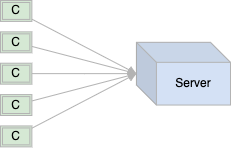
\includegraphics[width=6cm,height=6cm,keepaspectratio]{images/C-S.png}
                \caption{Client-Server Paradigma}
                \label{pic:cs}
            \end{subfigure}
            \begin{subfigure}[b]{0.4\textwidth}
                \centering
                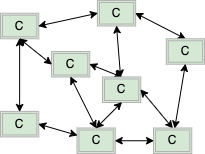
\includegraphics[width=6cm,height=6cm,keepaspectratio]{images/PtoP.png}
                \caption{Peer to Peer Paradigma}
                \label{pic:pp}
            \end{subfigure}
            \begin{subfigure}[b]{0.4\textwidth}
                \centering
                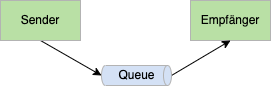
\includegraphics[width=7.5cm,height=7.5cm,keepaspectratio]{images/messagepassing.png}
                \caption{Message Passing Paradigma}
                \label{pic:messagepassing}
            \end{subfigure}
            \caption{Client-Server, Peer-to-Peer und Message Passing Interaktionsparadigma \cite{IEEE2015}}
            \label{pic:interactionparadigm}
        \end{figure}
        \\ 
        \begin{table}[hbt!]
            \begin{center}
                \begin{tabular}{| p{3cm} | p{12.75cm} | }
                    \hline
                        \textbf{Name} & \textbf{Beschreibung} \\
                    \hline
                        Client-Server (\ref{pic:cs}) & Basierend auf einer sehr einfachen Interaktion zwischen Clients und dem Server. Ein Client sendet eine Anfrage an den Server und erwartet dementsprechend eine Antwort. \\ 
                    \hline
                        \ac{PP} (\ref{pic:pp}) & Gegensatz zu Client-Server Konzept. Hierbei können Geräte sowohl als Client Dienste abfragen als auch als Server Dienste anbieten. \\ 
                    \hline
                        Message Passing (\ref{pic:messagepassing}) & Basierend auf einer einfachen Organisation in der ein Absender eine Nachricht mittels einer Warteschlange (Queue) an einen Empfänger weiterleitet. \\ 
                    \hline
                \end{tabular}
            \end{center}
            \caption{Interaktionsparadigmen nach \cite{IEEE2015}}
            \label{table:kommunikationdmodelle}
        \end{table}
        \\
        \pagebreak
        \linebreak
        Eine Analyse und detailliertere Darstellung der jeweiligen Ansätze kann der Ausarbeitung, aus der die Paradigmen verwendet wurden, entnommen werden.
        \\
        \linebreak
        Im Zusammenhang mit Architekturen, die in dem Bereich \acs{IoT} Anwendung finden, und Interaktionsparadigmen wird häufig zur Unterstützung 
        verschiedener Interaktionsmodelle auf Protokolle gesetzt, die Daten und Primitiven transportieren. Diese Kommunikationsmodelle sind in zwei 
        Bereiche, die ihre Anwendung in \ac{MtoM} finden, kategorisiert:
        \\
        \begin{itemize}
            \item \ac{SOAP}\footnote{Detailliertere Definition des Begriffs SOAP. \url{https://www.redhat.com/en/topics/integration/whats-the-difference-between-soap-rest} Abgerufen am 29.03.2022}: 
            Dabei handelt es sich um ein Standardprotokoll, das dafür entwickelt wurde, 
            um verschiedene Programmiersprachen auf verschiedenen Plattformen untereinander 
            kommunizieren zu lassen.
            \item \ac{REST}\footnote{Detailliertere Definition des Begriffs REST. \url{https://www.redhat.com/en/topics/integration/whats-the-difference-between-soap-rest} Abgerufen am 29.03.2022}: 
            Dabei handelt es sich um eine Reihe von Architekturprinzipien, die auf 
            die Anforderungen leichtgewichtiger Webdienste und mobiler Anwendungen abgestimmt sind. 
            Anfragen, die über diese Form gesendet werden, können in mehreren Formaten beantwortet 
            werden, darunter beispielsweise \ac{HTML}, \ac{XML} und \ac{JSON}.
        \end{itemize}
        Beide verfolgen das Ziel der Datenübermittlung zwischen Web-Anwendungen über eine Schnittstelle, das sogenannte \ac{API}.
        \acs{REST} Architekturen werden bei einem \acs{IoT}-Szenario aufgrund ihrer Simplizität und ihres Komforts bevorzugt. \cite{IEEE2015} 

    \subsection{Historische Entwicklung}
        Die ersten Konzepte zu dem heute bekannten \acs{IoT} liegen schon einige Jahrzehnte zurück. 
        Die historische Definition des \acl{IoT} wurde im Jahr 1999 von Kevin Ashton geprägt. Von der 
        Definition bis hin zum erstmaligen Einsatz bzw. zur Umsetzung eines Konzepts vergingen noch 
        ein paar Jahre. Ein kurzer Einblick in die chronologische Entstehung des \acs{IoT} ist der 
        folgenden Tabelle zu entnehmen: 
        \begin{table}[hbt!]
            \begin{center}
                \begin{tabular}{| p{3cm} | p{12.75cm} | }
                    \hline
                        \textbf{Jahr} & \textbf{Industrielle Beteiligung und Zuordnung} \\
                    \hline
                        1970 & Der erste Vorschlag zu miteinander verbundenen Geräten und Maschinen \\ 
                    \hline
                        1990 & John Romkey und Simon Hackett entwickelten den ersten Toaster, der über das Internet an- und ausgeschaltet werden konnte.\footnote{Geschichte to Romkey. \url{https://www.livinginternet.com/i/ia_myths_toast.htm} Abgerufen am 30.03.2022.} \\ 
                    \hline
                        1995 & Das Unternehmen Siemens leitete das erste Mobilfunkmodul ein, welches für die Kommunikation zwischen Maschinen zuständig ist (\acs{MtoM}-Technologie).\\ 
                    \hline
                        1999 & Die Definition des Begriffs \acs{IoT} von Kevin Ashton wurde veröffentlicht und von der Gesamtheit akzeptiert, als er bei \ac{PG} an den sogenannten \ac{RFID} Chips arbeitete. \acs{RFID}-Chips verwenden elektromagnetische Felder, die an Objekte angebracht sind, um diese identifizieren und verfolgen zu können. Ein solches System besteht aus einem Funktransponder, einem Funkempfänger und -sender. \\ 
                    \hline
                        2004 - 2005 & Der Begriff wurde in angesehenen Publikationen verwenden, darunter dessen von Boston Globe und The Guardian. \ac{ITU} veröffentlichte deren ersten Bericht über das Thema. \\ 
                    \hline
                        2008 - 2011 & Die Definitionen und Publikationen fanden erste Anwendungen in praktischen Umsetzungen. Gartner Inc. nahm den Begriff in ihre Recherche-Arbeiten mit auf. \\ 
                    \hline
                \end{tabular}
            \end{center}
            \caption{Historische Entwicklung vom \acl{IdD} \cite{Durga2020}}
            \label{table:iothistory}
        \end{table}
        \\
        \pagebreak
        \linebreak
        Mittlerweile ist das \acl{IdD} ein fester Bestandteil der Industrie, ebenso im privaten Umfeld. Viele 
        Szenarien und Konzepte werden erarbeitet und umgesetzt. Die Kommunikation von Maschinen untereinander 
        ist in der heutigen Zeit fester Bestandteil der Industrie und wird immer weiter ausgebaut. Forschergruppen sind daran interessiert, mehrere 
        Gebiete und Anwendungsbereiche innerhalb des \acs{IoT} zu erschließen. Stark vertreten ist dabei das \ac{FraunhoferIIS}

    \subsection{Ziele von \acs{IoT}}
    \label{subsec:ziele-iot}
        Die Definition von dem \acl{IdD} gibt die Richtung an, in die sich die Zielsetzung von 
        \acs{IoT} bewegt. Davon ist die Intention abzuleiten, dass die Lücke zwischen der realen und der 
        virtuellen Informationswelt so gering wie möglich gehalten bzw. zunehmend minimiert wird. 
        Dieser Informationsbedarf oder auch die Informationslücke besteht, da in der realen Welt Objekte, 
        Dinge und Gegenstände einen bestimmten Zustand vorzeigen. Ein Beispiel dazu ist „die Temperatur liegt bei 35 Grad Celsius“ 
        oder „das Licht ist an und hat 75 \% Helligkeit“. Diese Informationen sind in der virtuellen Welt nicht 
        ohne Weiteres verfügbar. 
        Das Bestreben demnach, welches auch zum Großteil im Bereich \acl{SH} abgedeckt wird, ist, dass 
        viele reale Gegenstände ihre Zustandsinformationen für die Weiterverarbeitung in der virtuellen 
        Welt beziehungsweise im Netzwerk zur Verfügung stellen. Diese Informationen können beispielsweise 
        Aussagen zu der aktuellen Nutzung, zur bestimmten Positionierung im Raum und 
        über die Alterung eines Gerätes geben. Diese Zustandsinformationen können dazu beitragen, dass die Nutzung des 
        Gegenstandes vom Anwender ausgewertet und so optimiert werden kann, z.B. durch die Erkennung 
        eines Defekts oder einer Automatisierung, damit die Ressource effizient genutzt wird. 

        %In einem weiteren Schritt können digitale Services als Teil des IoT die Parametrierung von 
        %Geräten so erleichtern und verbessern, dass sie auch dort geschieht, wo sie heute aus 
        %Kostengründen nicht stattfindet. Wichtige Schritte zu diesem Ziel sind:

        %die Standardisierung der Komponenten und Dienste im Internet der Dinge;
        %die Einführung einer einfach zugänglichen, sicheren und allgemeinen Netzwerkanbindung, geeignet für alle Geräte mit eingebautem Mikrocontroller;
        %die Reduktion der Kosten für in das IoT integrierte Teilnehmer (Gerätekosten, Inbetriebnahmekosten, Anschlusskosten etc.);
        %die Entwicklung von kostenarmen, automatisierten (bis hin zu autonomen) digitalen Services im Netzwerk, die den zusätzlichen Nutzen der Vernetzung realisieren.

\section{Smart Home}
\label{sec:smartHome}
    \acl{SH}, im Deutschen \textit{“intelligentes Zuhause“}, ist eine Domäne des \acs{IoT}. 
    Diese Rubrik der Anwendung widmet sich überwiegend dem Gebrauch von sämtlichen Haushaltsgeräten 
    und -einrichtungen. Ein kleiner Ausschnitt solcher Nutzgegenstände sind unter anderem Lampen, Kontaktsensoren, 
    Thermostate, Service-Roboter, Staubsauger-Roboter, Kühlschränke Geräte rundum die Haussicherheit. 
    \\ 
    Unter dem Oberbegriff \acl{SH} ist eine Weise zu verstehen, mit der die Erhöhung der Wohnqualität erzielt, 
    Energienutzung unter Verwendung vernetzter und fern steuerbarer Geräte effizienter gestaltet, Sicherheit gesteigert 
    und Abläufe verschiedener Prozessschritte automatisiert werden kann.
    \\ 
    Der Begriff \textit{intelligentes Zuhause} wird verwendet, wenn die Haustechnik und Haushaltsgeräte untereinander 
    vernetzt sind. Die Definition im deutschen Gebrauch, welche nach (Strese et al. 2010) in der Untersuchung im Rahmen 
    der wissenschaftlichen Begleitung zum Programm \textit{„Next Generation Media (NGM) des Bundesministeriums für Wirtschaft und Technologie“} 
    aufgegriffen wird, lautet wie folgt: 
    \begin{quote}
        „Das Smart Home ist ein privat genutztes Heim (z.B. Eigenheim, Mietwohnung), in dem die zahlreichen Geräte der 
        Hausautomation (wie Heizung, Beleuchtung, Belüftung), Haushaltstechnik (wie z.B. Kühlschrank, Waschmaschine), 
        Konsumelektronik und Kommunikationseinrichtungen zu intelligenten Gegenständen werden, die sich an den 
        Bedürfnissen der Bewohner orientieren. Durch Vernetzung dieser Gegenstände untereinander können neue 
        Assistenzfunktionen und Dienste zum Nutzen des Bewohners bereitgestellt werden und einen Mehrwert 
        generieren, der über den einzelnen Nutzen der im Haus vorhandenen Anwendungen hinausgeht.“ \cite{strese.2010m}
    \end{quote}
    Eine vergleichbare Definition wurde zu späterem Zeitpunkt durch eine Literaturrecherche publiziert. Diese beschreibt 
    die zugrunde liegende Thematik weniger aus Anwendersicht, sondern widmet sich vielmehr dem System und der Konnektivität. 
    \begin{quote}
        „A smart home is a place with heterogeneous systems to many
        front devices with the support of embedded information and
        communication architectures[...]“ \cite{Balakrishnan2018}
    \end{quote}
    Den beiden Definitionen ist zu entnehmen, dass die Kernaussage eine ähnliche ist, es jedoch in Büchern, Fachartikeln, 
    Publikationen an Universitäten und in den verbreiteten Medien bis heute keine durchgängige gibt. Aus der 
    einschlägigen Literatur wird ersichtlich, dass viele Synonyme für die Benennung der Thematik verwendet werden, darunter 
    beispielsweise \cite{strese.2010m}:
    \\
    \linebreak
    \pagebreak
    \begin{itemize}
        \item Connected Home
        \item Elektronisches Haus
        \item Intelligentes Haus (engl. Smart House)
        \item Smart Living
        \item Home of the Future 
    \end{itemize}
    Eine elementare Information im Zusammenhang dieser Arbeit ist die Verwendung des Begriffs \textit{intelligentes Büro}, die 
    ebenso in den Kontext des \acl{SH} gehört. Hierbei wird lediglich die Räumlichkeit im unternehmerischen Jargon verwendet, 
    die ebenso eine Grundlage für die Verwendung von Komponenten des \acl{SH} bietet. Im Abschnitt (\ref{subsec:smartoffice}) wird 
    nochmals konkret darauf eingegangen.
    \\
    Es wird deutlich, dass die Verwendung des Begriffs als auch die zugrunde liegenden technischen Verfahren 
    weiträumig einsetzbar sind und deshalb die Begriffsdefinition nicht eindeutig festgehalten werden kann. 
    
    \subsubsection*{Teilsysteme des \acl{SH}}
    \label{subsubsec:teilsystemeSH}
        Der primäre Anwendungsbereich des \acl{SH} ist die Automatisierung häuslicher Prozesse. Dadurch sollen dem Nutzer 
        in vielerlei Hinsicht Aufwände erspart und Informationen zentralisiert angezeigt werden. Die Hausautomatisierung 
        umfasst eine Menge von Teilsystemen. Ein Ausschnitt dieser Teilsysteme ist der folgenden tabellarischen Auflistung zu entnehmen: 
        \begin{table}[hbt!]
            \begin{center}
                \begin{tabular}{| p{3cm} | p{12.75cm} | }
                    \hline
                        \textbf{Segment} & \textbf{Beschreibung} \\
                    \hline
                        Licht & Beleuchtung, Lichtmanagement/Szenarien, Storen/Rollos \\ 
                    \hline
                        Zutritt & Zutrittskontrolle, Klingelanlage, Schlösser, Anwesenheits- und Bewegungserfassung \\ 
                    \hline
                        Überwachung & Technische Alarme: Feuer, Rauch, Gas; Intrusion: Glasbruchmelder, Video; Babyphon, Urlaubswachschutz \\ 
                    \hline
                        Notfall & Sprinkleranlage, unabhängige Stromversorgung, Fluchtwegsystem \\ 
                    \hline
                        Metering & Verbrauchszähler für Strom, Gas, Wasser, Wärme, uvm. \\ 
                    \hline 
                        Konsumelektronik & TV, Internet, Smartphones, Tablets, Spielekonsolen etc. \\
                    \hline
                        Hausgeräte & Kühlschrank, Waschmaschine, Staubsauger, Service-Roboter; Hausgeräte-monitoring, -diagnostik, und -fernbedienung \\
                    \hline
                        Heimlogistik & Einkaufs- und Speiseplanung, häusliche Dienste \\ 
                    \hline
                        Hobby & Haustierversorgung, Aquarienmanagement, etc. \\
                    \hline
                        Mobilität & PKW mit Diagnostik, Navigationssystem mit local based services, Info-/Entertainmentangebote etc. \\ 
                    \hline
                \end{tabular}
            \end{center}
            \caption{Teilsysteme des Smart Home \cite{strese.2010m}}
            \label{tab:teilsysteme}
        \end{table}
        \\
        \linebreak
        Die Ausstattung des Smart Home mit Intelligenz und die Vernetzung der Teilsysteme untereinander haben zum Ziel, die Aufgaben möglichst 
        autonom mit wenig übergeordneter, zentraler Steuerung abzuarbeiten. 
        Dabei müssen die erzeugten als auch erforderlichen Daten mit anderen 
        Komponenten des Gesamtsystems ausgetauscht werden. 
        \\
        Eine mögliche Vernetzung und auch Verwendung solcher Komponenten wird in folgender Abbildung (\ref{pic:szenarien-smarhome}) 
        skizziert. Diese Grafik dient als grobe Übersicht potenzieller Anwendungsszenarien, repräsentiert jedoch nicht alle Möglichkeiten der Anwendung. %ist allerdings nicht als vollständig zu interpretieren. 
        \begin{figure}[hbt!]
            \centering
            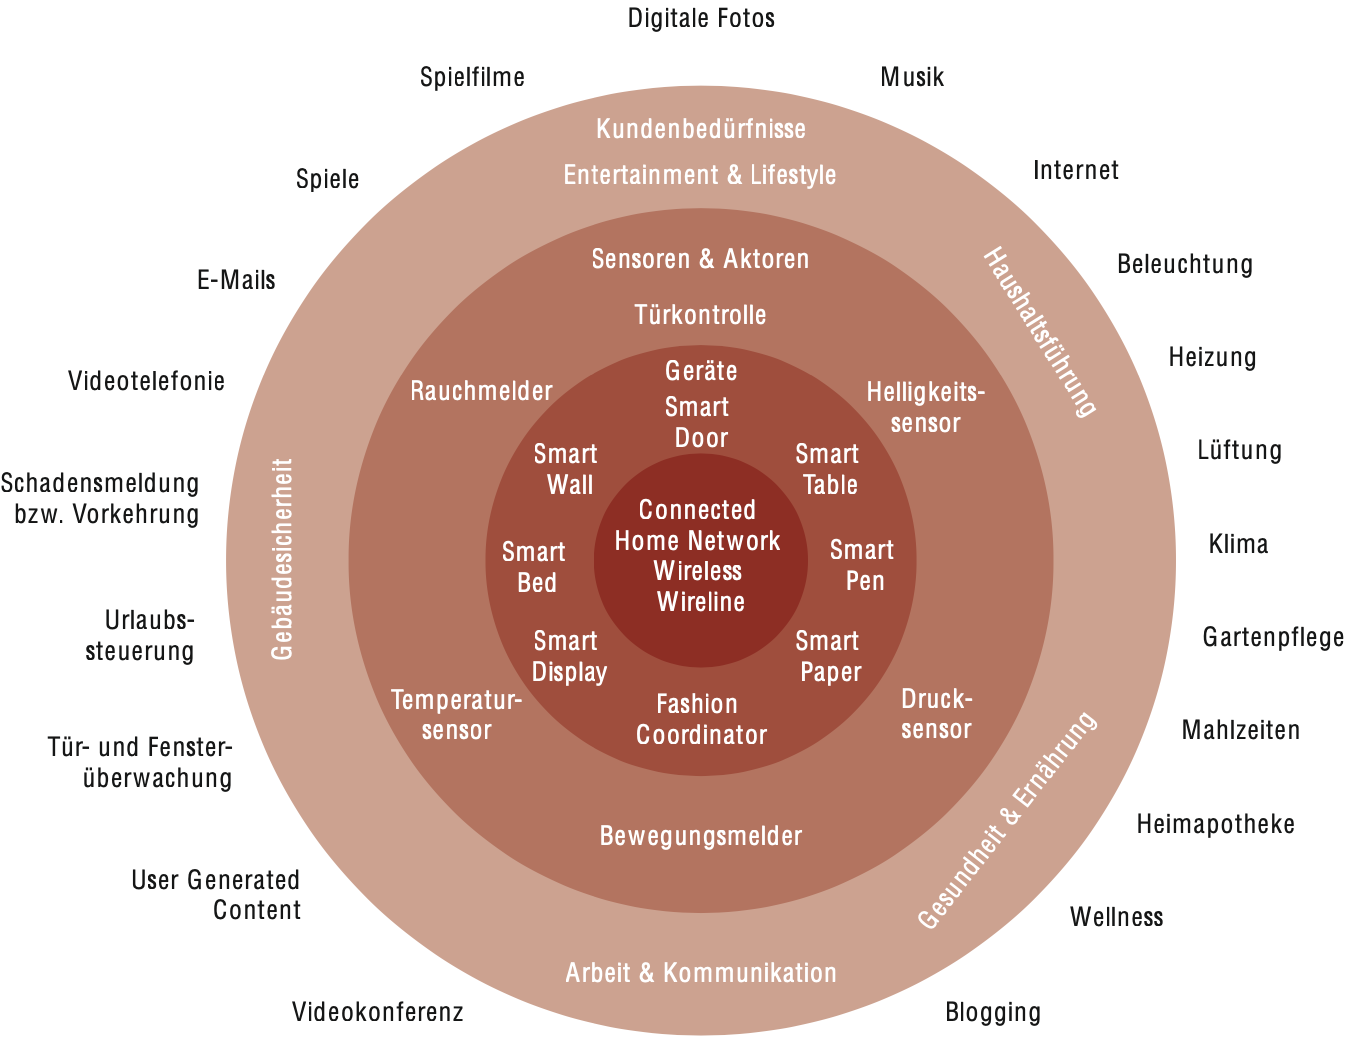
\includegraphics[width=15cm,height=15cm,keepaspectratio]{images/Anwendungsszenarien_SH.png}
            \caption{Mögliche Anwendungsszenarien im Smart Home \cite{strese.2010m}}
            \label{pic:szenarien-smarhome}
        \end{figure}
        \\
        Darüber hinaus gibt es weitaus mehr Anwendungsszenarien, beziehungsweise werden diese in der Abbildung 
        (\ref{pic:szenarien-smarhome}) in einem Überbegriff zusammengefasst.
        Ein immer bedeutenderes Anwendungsszenario ist die Kopplung 
        von Robotern jeglicher Art, darunter die schon weit verbreiteten Staubsaugerroboter oder 
        vor allem Service-Roboter, die immer mehr in die Thematik des \acl{SH}  zu integriert versucht werden. 
        
    \subsubsection*{Einordnung von Smart Home in das Internet der Dinge}
    \label{subsubsec:smartHome-IoT}
        Im Konsumentenmarkt wird die Technologie des \acs{IoT} in Produkten eingesetzt, die 
        das Konzept des \acl{SH} verfolgen.  
        Diese beinhalten Haushaltsgeräte und -ausstattung, wie beispielsweise Thermostate, Sensoren, 
        Sicherheitssysteme und Lampen, die mehrere Systeme und Übertragungstechnologien 
        unterstützen. Dazu zählen unter anderem Plattformen, darunter Google Nest, Apple HomeKit 
        und Amazon Alexa uvm., ebenso die Übertragungstechnologien, die im Abschnitt (\ref{sec:technologien}) 
        aufgegriffen werden.
        Weitere Beispiele sind der Tabelle (\ref{tab:teilsysteme}) zu entnehmen. 
        \begin{figure}[hbt!]
            \centering
            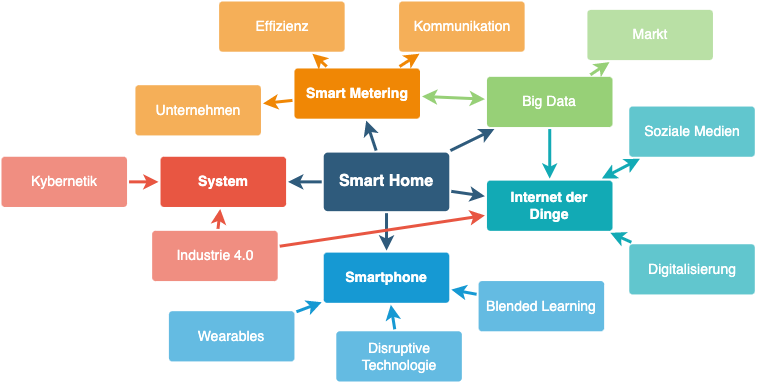
\includegraphics[width=15cm,height=15cm,keepaspectratio]{images/SH-Mind_Map.png}
            \caption{Technologische Einordnung von Smart Home in Verbindung zu IoT \cite{shmindmap2021}}
            \label{pic:mindmap_SH-IoT}
        \end{figure}
        \\
        %\linebreak
        Die Abbildung (\ref{pic:mindmap_SH-IoT}) zeigt die Verbindungen als auch die Beziehungen von \acl{SH} 
        zu anderen Technologien. Hier wird deutlich, dass im Bereich des \acl{SH} viele Fragestellungen 
        thematisiert werden können, die andere Themenbereiche tangieren. Mit inbegriffen ist zum Beispiel die 
        Komponente Smartphone, da dieses genutzt wird, um als Fernbedienung zu fungieren und Prozesse und 
        Automationen anzeigen und überwachen zu können. Der Bereich des Smart Metering\footnote{Smart Metering ist das computergestützte Messen, Ermitteln und Steuern von Energieverbrauch und -zufuhr. \url{https://wirtschaftslexikon.gabler.de/definition/smart-metering-53998} Abgerufen am 06.04.2022} 
        deckt die Messung von Verbrauchsdaten ab. Dabei handelt es sich um intelligente Messsysteme, die 
        Daten zum Verbrauch, darunter Strom, Gas und Wasser, erheben und diese von den jeweiligen Anbietern zur 
        Rechnungsstellung genutzt werden. Ein Beispiel dazu ist ein digitaler intelligenter Stromzähler mit 
        direkter Kommunikationsmöglichkeit zum Anbieter selbst.
        \\
        \linebreak
        Der Aufbau eines \acl{SH} ist architektonisch ähnlich zu dem Grundprinzip einer \acs{IoT}-Lösung. Die 
        Veranschaulichung des zugrunde liegenden Aufbaus ist der Abbildung (\ref{pic:skizze_iot}) zu entnehmen. 
        \\
        Um die Bezugspunkte zu \acs{IoT} und die Einordnung zu untermauern, wird in folgendem Abschnitt auf 
        die Funktionsweise von \acl{SH} eingegangen. 

    \subsubsection*{Funktionsweise eines \acl{SH}}
    \label{subsubsec:funktionsweise}
        Ein \acl{SH} System besteht aus mehreren Teilsystemen, die in der Regel aus verschiedenen Komponenten bestehen. 
        Wichtige Elemente eines grundlegenden Aufbaus sind die Endgeräte, die sogenannten Aktoren, Eingabegeräte, 
        Sensoren, Gateway und die Vernetzung über Funk, Kabel oder Stromnetz. Die Endgeräte sind die Ausgabegeräte, die 
        über die intelligente Steuerung angesprochen werden können. Darunter zählen zum Beispiel 
        LED-Lampen, Rolläden, Lüftungsanlagen, Lautsprecher, Fernseher, Waschmaschinen und jegliche Arten von 
        Service-Robotern. Eingabegeräte sind die Schnittstelle zwischen der Interaktion des Nutzers und des 
        Smart Home Systems. Das können Wandschalter, Touch-Displays, Fernbedienungen, Smartphones und Regler sein. 
        Mithilfe dieser Schnittstelle können Zustände und Aktionen an den Endgeräten ausgelöst werden. Bei einer 
        fehlenden Verbindung zwischen den Steuerelementen sind diese trotzdem noch über direkte Schaltbefehle steuerbar. 
        Damit die Zustände ebenso digitalisiert werden können und dem System zur Verfügung stehen, werden Sensoren 
        benötigt. Diese greifen die physikalischen oder elektronischen Eigenschaften des Endgerätes ab, um die 
        Zustände zu ermitteln. Das Gateway repräsentiert die zentrale Steuereinheit, auf dem die Sensordaten 
        eingehen und die Sendung von Befehlen an die Aktoren stattfindet. Ebenso ermöglicht das Gateway die 
        Kommunikation der Endgeräte und Sensoren untereinander. Eine mögliche Internetverbindung zwischen 
        dem Gateway und einer zentralen Plattform, die über die Cloud erreichbar ist, kann ebenso hergestellt werden. 
        Je nach Gerät kann über das Gateway auch eine direkte Steuerung einzelner Elemente stattfinden. Das letzte 
        Element, die Vernetzung, ist für die Verbindung aller Elemente zuständig. Hierfür kommen verschiedene 
        Protokolle, die unter anderem in Abschnitt (\ref{sec:technologien}) beschrieben werden, 
        per Funk, Kabel oder Stromnetz zum Einsatz. % https://www.verbraucherzentrale.de/wissen/umwelt-haushalt/wohnen/smart-home-das-intelligente-zuhause-6882#:~:text=Darunter%20fallen%20zum%20Beispiel%20Heizk%C3%B6rperregler,aus%20einem%20oder%20mehreren%20Eingabeger%C3%A4ten.
        \\
        Ein exemplarischer Aufbau der Komponenten ist der folgenden Abbildung zu entnehmen:
        \begin{figure}[hbt!]
            \centering
            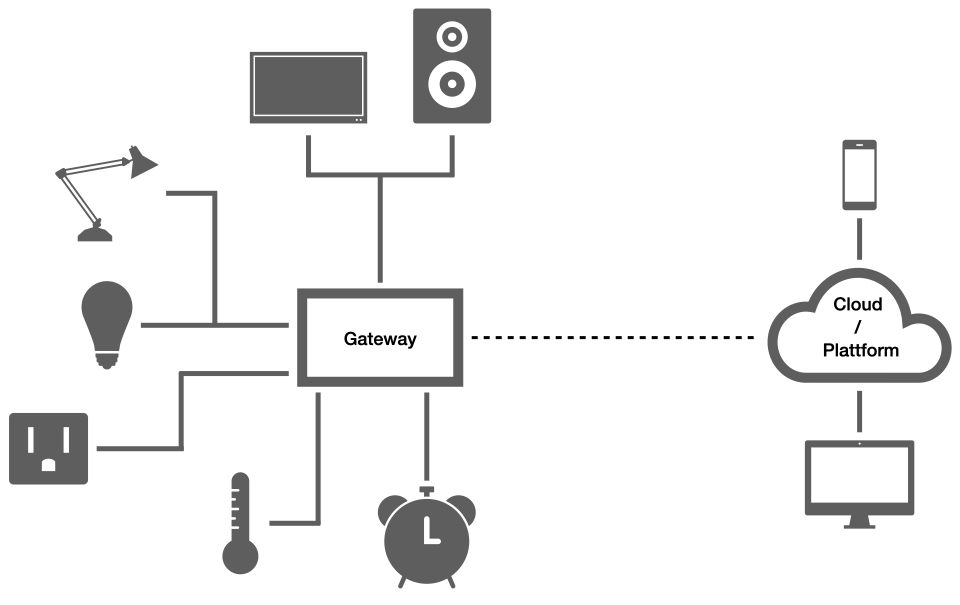
\includegraphics[width=13cm,height=13cm,keepaspectratio]{images/smart_home_connection.png}
            \caption{Aufbau und Funktionsweise einer Smart Home Infrastruktur}
            \label{pic:aufbau_SH}
        \end{figure}

    % Quelle: https://animus.de/smart-office Abgerufen am 18.05.2022
    \subsection{Smart Office - Intelligentes Büro}
    \label{subsec:smartoffice}
        Ein Smart Office, im Deutschen intelligentes Büro, ist ein konkreter Anwendungsbereich des Smart Home. 
        Während das Smart Home vorwiegend von der Verbesserung des Komforts, der Einsparung von Energiekosten,  
        der Optimierung des Wohlbefindens im privaten Wohnraum und der Erleichterung des Alltags des Nutzers handelt, 
        zielt das Smart Office darauf ab, das Wohlbefinden und die Produktivität der Mitarbeiter zu steigern. Weitere 
        wichtige Punkte sind neben den beiden aufgeführten auch die Erhöhung der Sicherheit der Büroräume und der 
        Nachhaltigkeit durch z.B. Reduzierung des Stromverbrauchs. In diesem Zusammenhang spielt die Automation 
        von Gebäudemanagement- und die damit verbundenen Sicherheitssysteme eine große Rolle. 
        \\
        \linebreak
        Viele Funktionalitäten und Vorteile sind deckungsgleich zu denen des Smart Home. Durch intelligente Geräte, Aktoren und 
        Sensoren ist die Steuerung von Licht, Raumtemperatur etc. möglich. Hervorzuheben ist unter anderem die mögliche Zutrittskontrolle 
        per Gesichtserkennungssysteme, die an zentraler Stelle mit weiteren Komponenten kommunizieren und beliebige zusätzliche Schritte 
        einleiten können. Ebenso zu nennen ist der Aspekt in Richtung Gebäudesicherheit und deren Ausbau, denkbar in Form von intelligenten 
        Feuer- und Wassermeldern oder weiteren Maßnahmen, die durch Automationen abgebildet werden können. 
        \\
        In unserer heutigen Zeit ist die Nachhaltigkeit und Ressourceneffizienz von immer größerer Bedeutung.
        Automatische Abschaltungen von Beleuchtungen, Kaffeemaschinen, Monitoren oder anderen Geräten durch 
        Präsenz- und Bewegungsmelder oder Remotesteuerungsoptionen können Ressourcen- und Energieeinsparungen umsetzen. 
        
    \subsection{Historische Entwicklung}
    \label{subsec:entwicklung_sh}
        Im Bereich des \acl{SH} wurde im Jahr 1975 die erste Netzwerktechnologie für Hausautomationen 
        präsentiert und vermarktet. Bekannt wurde diese unter dem Namen \textit{X10}\footnote{\url{https://de.wikipedia.org/wiki/X10_(Protokoll)} - X10 Protokoll Erklärung. Abgerufen am 06.04.2022}. 
        Dabei handelt es sich um ein stromleistungsbasiertes Netzwerkprotokoll zur Gebäudeautomation. Die 
        Schaltsignale werden über die Hausinstallation, das Stromnetz des Hauses, transportiert. Eingeführt wurde die 
        Technologie von dem Unternehmen Busch-Jaeger unter dem Namen \textit{Timac X10}. Es zeichnete sich durch die 
        einfache Konfiguration und dessen interessante Funktionen zu diesem Zeitpunkt aus \cite{aschendorf2014energiemanagement}. % URL zur Zitierquelle: https://books.google.de/books?id=-y8pBAAAQBAJ&dq=Bernd+Aschendorf:+Energiemanagement+durch+Geb%C3%A4udeautomation.+Vieweg,+2014,+ISBN+978-3-8348-0573-7,+S.+55.&lr=&hl=de&source=gbs_navlinks_s 
        Die Weiterentwicklung des Systems, Timac X10, fand im Jahre 1998 statt, indem von Busch-Jaeger ein neues 
        Produkt Namens \textit{Powernet EIB} in Deutschland eingeführt wurde. Dieses baute ebenso auf dem grundlegenden 
        Netzwerkprotokoll X10 auf und fügte sich einwandfrei in den europäischen Installationsbus (EIB/KNX) ein \cite{busch-jaeger}. 
        KNX ist ein Bussystem zur Gebäudeautomation, welches basierend auf dem EIB weiterentwickelt wurde. Es 
        zählt heute noch zu den kabelgebundenen Standards. Im Jahre 2001 eröffnete die Fraunhofer IMS in Kooperation 
        mit der Universität Duisburg-Essen die Fraunhofer-inHaus-Forschungsanlage \cite{fraunhofer-forschungsanlage}. 
        Innerhalb dieser Institution erforschten, entwickelten, testeten und demonstrierten Dienstleister, Hersteller und Nutzer 
        mit dem Fraunhofer-Institut und der Universität neue Systemlösungen und weitere Produktkomponenten sämtlicher Arten 
        im Bereich des Wohnens. Anfang des Jahres 2005 wurde die deutsche Telekom in dem \acl{SH} Bereich aktiv und 
        präsentierte der Öffentlichkeit ein vollständig vernetztes, „intelligentes“ Musterhaus in Berlin, das sogenannte 
        \textit{T-Com-Haus}. Anfang des Jahres 2012 wurde das \ac{BMWK} im Sektor des \acl{SH} aktiv. Seitdem fördert die 
        Behörde das \textit{„Zertifizierungsprogramm Smart Home + Building“}, bei dem Forschungen im Bereich des \acl{SH} 
        von Vertretern akademischer Einrichtungen und Industrieunternehmen %, die in diesem Segment unterwegs sind, 
        durchgeführt werden. Ziele dabei sind unter anderem die Erstellung von Standards und Prüfsiegeln für 
        systemübergreifende Interoperabilität der Geräte eines \acl{SH} \cite{vde-smartAndBuilding}. 
        2013 präsentierte die deutsche Telekom neue Lösungen in einem weiteren Musterhaus in Darmstadt. 
        Darin finden sich mehrere Komponenten und Vernetzungen als im Berliner Modell \cite{telekom_SH}, so die 
        Nutzung verschiedener Funkstandards, die es ermöglichen, intelligente Geräte 
        unterschiedlichster Hersteller zu konfigurieren und über ein Smartphone, Tablet oder Computer zu kontrollieren 
        und zu steuern \cite{telekom_SH}. Die Auswirkungen der rasanten Entwicklung dieser Technologie trieben das 
        Interesse in die Höhe, sodass 2014 und 2015 die Technologie das Hauptthema der \ac{IFA} bei vielen 
        Ausstellern war.
        \\
        Bis heute wird in dem Segment des \acl{SH} geforscht und immer weitere Funktionalitäten entwickelt. Der Trend 
        der Nutzung von intelligenten Geräten ist weiter zunehmend. Die Marktsituation und der aktuelle Ist-Stand 
        wird in dem Abschnitt Marktanalyse (\ref{sec:marktanalyse}) nochmals aufgegriffen und mit Statistiken und Umfragen belegt.
    %\pagebreak

    \subsection{Ziele von Smart Home} % https://www.bigdata-insider.de/was-ist-smart-home-a-809018/ 
    \label{subsec:ziele_sh}
        Die Ziele der intelligenten Vernetzung sind in erster Linie diejenigen, die die 
        großen Domänen abdecken \cite{goals-smarthome}:
        \begin{itemize}
            \item Komfort (Steuerung, Fernbedienung, Delegation und Automationen)
            \item Energie- und Kosteneffizienz
            \item Sicherheit (Überwachung)
        \end{itemize}
        Allgemein lässt sich der Komfort durch die entfernungsunabhängige, bequeme Steuerung von Licht, Heizung, Unterhaltungselektronik, 
        Service-Robotern und vielen weiteren Geräten steigern. 
        Hierfür spielen beispielsweise Smartphones, zentrale Steuerungsgeräte und Tablets eine wichtige Rolle. 
        Diese fungieren ähnlich wie eine herkömmliche Fernbedienung. Es können ebenso Prozesse 
        automatisiert oder durch ein bestimmtes vorgegebenes Ereignis, welches 
        eintreten kann, angestoßen werden. Mit diesen Automationen können gewünschte Wohnbedingungen zu 
        bestimmten Anlässen und Zeiten erzeugt werden. Beispielsweise kann die Heizung vor Eintreffen reguliert 
        werden, um die optimale Temperatur zu erreichen. Die Steuerung von 
        Geräten spielt gleichermaßen eine Rolle in den Bereichen der Energie- und Kosteneffizienz und der Sicherheit. 
        \\
        \linebreak
        Durch das Verbinden mehrerer Komponenten mithilfe einer Automation können Energiekosten verringert werden, wenn 
        bspw. ein Temperaturabfall durch ein offenes Fenster von Sensoren gemessen wird und diese ein Signal übermitteln. 
        Dementsprechend kann die Heizung für den Zeitraum 
        ausgeschaltet oder reguliert werden, um überflüssige Wärmeerzeugung zu vermeiden. Weitere Einsparungen können durch 
        das Ausschalten von aktuell nicht benötigten Ressourcentypen, wie z.B. Elektrogeräten 
        oder LED-Lampen, vorgenommen werden.
        \\
        \linebreak
        Zuletzt ist die Erhöhung der Sicherheit und das Überwachen von Eingängen und Fenstern zu nennen.
        Die Bewegungsmelder und Sensoren können Aktivitäten registrieren und sind Auslöser für die Weitergabe 
        der Information an den Eigentümer. Zusätzlich können mit Kameras Objekte überwacht werden, beispielsweise ein Haustier, das 
        kurze Zeit alleine zu Hause ist oder es können Einbruchsversuche registriert und gemeldet werden. Auch eine Alarmierung bei 
        Flutung des Kellers oder bei Hausbrand sind denkbar.
        \\
        \linebreak
        Die Geräte im \acl{SH} erreichen weitestgehend diese Ziele und werden stetig weiterentwickelt, verbessert und um neue 
        Funktionalitäten ergänzt.

\section{Technologien}
\label{sec:technologien}
    Die bereits angesprochene Kommunikation und Vernetzung zwischen Geräten basiert im Allgemeinen auf 
    diversen Protokollen. Um diese Datenbewegung und Kommunikation besser verstehen zu können, werden im 
    Folgenden bekannte Protokolle erwähnt und aufgeführt und eines der meist verwendeten näher betrachtet. 
    Um einen Vergleich herzustellen, wird ein vergleichbares Protokoll begutachtet. Diese werden dann zum 
    Abschluss gegenübergestellt. 

    \subsection{Übertragungsmethoden}
    \label{subsec:netzwerkprotokolle}
    Allgemein gibt es im Bereich des \acl{SH} mehrere Methoden und Möglichkeiten, die Objekte miteinander zu vernetzen. 
    Dazu gehören Protokolle über Bluetooth, Ethernet, WLAN, Bussysteme, Funk und Stromleitung. 
    Jeder Hersteller setzt diese abhängig von seinem Produkt passend ein. Proprietäre Systeme funktionieren nur über eine 
    Übertragungsmethode. So erzwingen die Hersteller die Nutzung einer Produktlinie bzw. den Kauf von Elementen eines 
    einheitlichen Systems. Geräte, die die Möglichkeiten besitzen, über mehrere Protokolle 
    zu kommunizieren, sind flexibler einsetzbar und mit mehreren Plattformen und Geräten kompatibel.
    Grundlegend werden mit diesen Übertragungsmethoden Netzwerke erstellt, über das die Geräte in einem \acl{SH} kommunizieren können.
    \\
    \linebreak    
    Die Auflistung der zum aktuellen Zeitpunkt am meist verwendeten Übertragungsmethoden dient 
    lediglich als Einblick in die verschiedensten Ausprägungen der Kommunikationstechnologie.   
    Demnach wird im Rahmen dieser Arbeit das Thema nicht ausführlich vertieft.
    Ein Ausschnitt der populärsten Übertragungsmethoden wird in folgender Tabelle aufgelistet\footnote{Auswahl von derzeit verwendeten Übertragungsmethoden. \url{https://de.wikipedia.org/wiki/Smart_Home\#Übertragungsmethoden} Abgerufen am 02.04.2022}. 
    %ZigBee? Erläuterung etwas detaillierter?

    % https://www.bigdata-insider.de/so-laeuft-der-datenaustausch-zwischen-edge-und-cloud-a-1097887/ 